\documentclass[12pt, a4papre]{article}
\usepackage[catalan]{babel}
\usepackage[unicode]{hyperref}
\usepackage{amsmath}
\usepackage{amssymb}
\usepackage{amsthm}
\usepackage{xifthen}
\usepackage{listings}
\usepackage{float}
\usepackage{graphicx}

\newcommand{\norm}[1]{\lvert #1 \rvert}
\graphicspath{ {./Images/} }

\hypersetup{
    colorlinks = true,
    linkcolor = blue
}

\author{Daniel Vilardell}
\title{Entregable ICOM}
\date{}

\begin{document}
	\maketitle
	\textbf{a)} En aquest apartat demostrarem que $b_y(t) = \frac{1}{2} b_s(t)  * b_h(t)$.
	
	Sabem en primer lloc que el resultat de passar un senyal $x(t)$ per un filtre amb resposta impulsional $h(t)$ es $y(t) = x(t)*h(t)$. Per tant
	
	\[
		Y(f) = X(f)H(f) \implies Y^+(f) = X^+(f)H^+(f) \implies
	\]
	\[
		\implies \frac{1}{2} B_y(f)= \frac{1}{2}B_x(f)\frac{1}{2}B_h(f) \implies B_y(f)= \frac{1}{2}B_x(f)B_h(f) \implies
	\]
	\[
		\implies b_y(t) = \frac{1}{2}b_x(t)*b_h(t)
	\]
	
	
	\textbf{b)} Podem veure que si considerem una senyal $\alpha j sign(f)$ i ens restringim al domini $ [f_0 - B, f_0 + B]$ ens dona com a resultat un pols rectangular centrat al punt $f_0$, d'amplitud $\alpha$ i de ample de banda $B$. Per tant, si ho desplacem $f_0$ unitats cap a l'esquerra obtindrem
	
	\[
		B_h(f) = \prod\left(\frac{f}{B}\right)
	\]
	
	\textbf{c)} Savem com hem vist a teoria que $B_y(f) = \frac{1}{2}B_x(f)B_h(f)$. Aplicarem aquesta formula per a trobar el resultat demanat.
	
	\[
		B_y(f) = \frac{1}{2}B_x(f)B_h(f) = \frac{\alpha j}{2} (I_x(f) + jQ_x(f)) \prod\left(\frac{f}{B}\right)
	\]
	Com que l'ample de banda de $i_x(t)$ i de $q_x(t)$ es $B$, ens dona el següent.
	\[
		B_y(f) = \frac{\alpha}{2} (I_x(f) + jQ_x(f))e^{j\frac{\pi}{2}} = \frac{\alpha}{2}B_x(f)e^{j\frac{\pi}{2}}
	\]
	
	També podem concluir que $b_y(t) =  \frac{\alpha}{2}b_x(t)e^{j\frac{\pi}{2}}$
	\\
	
	\textbf{d)} 
	
	\begin{figure}[H]
		\begin{center}
		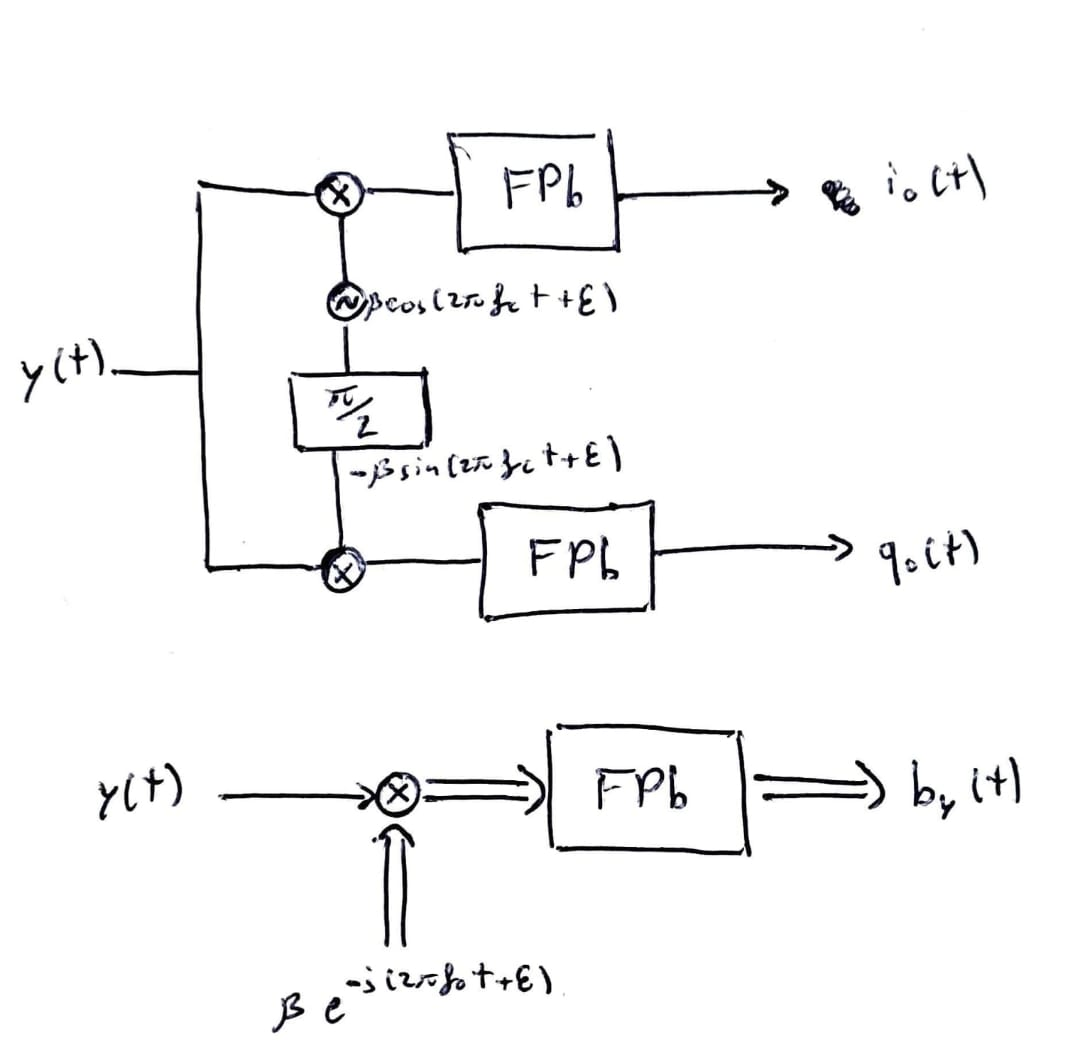
\includegraphics[width=110mm]{Entr1.jpeg}
		\caption{Diagrama de blocs del demodulador $I\&Q$}
		\end{center}
	\end{figure}
	
	\textbf{e)} Usarem la expressió complexa del demodulador I\&Q per a fer els calculs i obtenir $b_0(t)$. Partim de la senyal $y(t)$. A partir d'aquesta obtenim despres de multiplicar per $\beta e^{-j(2\pi f_ct + \varepsilon)}$ ens dona $ \beta y(t)e^{-j(2\pi f_ct + \varepsilon)}$. Després de passarho pel filtre passa baix ens donarà $ \beta b_y(t) e^{-j\varepsilon}$. D'aquí podem concluir que
	
	\[
		b_0(t) = \beta b_y(t) e^{-j\varepsilon} = \frac{\alpha\beta}{2}b_x(t)e^{j\frac{\pi}{2}}e^{-j\varepsilon} = \frac{\alpha\beta}{2}b_x(t)e^{j(\frac{\pi}{2} - \varepsilon)}
	\]
	
	\textbf{f)} Deduirem el resultat partint de que $b_0(t) = \frac{\alpha\beta}{2}b_x(t)e^{j(\frac{\pi}{2} - \varepsilon)}$ i $b_x(t) = i_x(t) + jq_x(t)$.
	
	\[
		b_0(t) = \frac{\alpha\beta}{2}b_x(t)e^{j(\frac{\pi}{2} - \varepsilon)} =  \frac{\alpha\beta}{2}(i_x(t) + jq_x(t))e^{j(\frac{\pi}{2} - \varepsilon)} = 
	\]
	\[
		= \frac{\alpha\beta}{2}((i_x(t)\cos(\frac{\pi}{2} - \varepsilon) - q_x(t)\sin(\frac{\pi}{2} - \varepsilon)) + j(q_x(t)\cos(\frac{\pi}{2} - \varepsilon) + i_x(t)\sin(\frac{\pi}{2} - \varepsilon))) =
	\]
	\[
		= i_b(t) + jq_b(t)
	\]
	Per tant d'aquí podem deduir que
	
	\[
		i_b(t) =  \frac{\alpha\beta}{2}(i_x(t)\cos(\frac{\pi}{2} - \varepsilon) - q_x(t)\sin(\frac{\pi}{2} - \varepsilon))
	\]
	\[
		 q_b(t) = \frac{\alpha\beta}{2}(q_x(t)\cos(\frac{\pi}{2} - \varepsilon) + i_x(t)\sin(\frac{\pi}{2} - \varepsilon))
	\]
	
	\textbf{g)} Per a que $b_0(t) = b_x(t)$ s'ha de donar que $b_0(t) = \frac{\alpha\beta}{2}b_x(t)e^{j(\frac{\pi}{2} - \varepsilon)}$ i per tant $\beta = \frac{2}{\alpha}$ i $\varepsilon$ ha de ser de la forma $\varepsilon = \frac{\pi}{2} + k2\pi$ on $k \in \mathbb{Z}$. Un possible valor per tant seria $\varepsilon = \frac{130689}{2}\pi$.
\end{document}










